\documentclass[
    bibstyle = apa,
    mathfont = arev
]{spArticle}
\spAuthor{Sweet Pastry}
\spAffiliation{Fudan University}
\spTitle{\texttt{spArticle} Document}
\spAbstract{This document provides comprehensive instructions for the \LaTeX\ class file \texttt{spArticle}. The accompanying text and source code are located within the same directory. The \texttt{spArticle} class is designed to offer a fully packaged article template, enabling users to focus exclusively on content creation without the need to manage complex \LaTeX\ code or address grammatical issues. It incorporates nearly all packages commonly utilized by students in scientific and engineering disciplines, allowing users to avoid adding extra code in the preamble. \texttt{spArticle} is not tailored specifically for scientific thesis writing; instead, it serves as a versatile template suitable for personal notes, assignments, and similar applications.}


\begin{document}
    \section{How to Use}
        \subsection{\texttt{.tex} File}
            To use this template, first download the class file \texttt{spArticle.cls} and create a new \texttt{.tex} file. In that file, include the following code snippet to specify the essential information for your article.
            \begin{Verbatim}[xleftmargin=-50pt]
                \documentclass[
                    author = author,
                    affiliation = affiliation,
                    date = \today,
                    bibstyle = ieee,
                    title = title,
                    abstract = abstract,
                    ref = ref
                ]{spArticle}
            \end{Verbatim}

            If your title, name, affiliation, or abstract is very long or contains advanced elements like mathematical symbols, you may encounter compilation issues \footnote{This happens because any values passed to the \texttt{.cls} file via the \texttt{\textbackslash documentclass} command are processed before certain macros are loaded.}. In such cases, I recommend avoiding the use of \texttt{\textbackslash documentclass} options to set private variables. Instead, please use the specialized commands in the preamble provided below.
            \begin{Verbatim}[xleftmargin=-70pt]
                \spAuthor{Your Name}
                \spAffiliation{Your Affiliation}
                \spDate{If You want set time manually}
                \spTitle{Your Title}
                \spAbstract{You can write a lot here}
            \end{Verbatim}

            After providing all the necessary information, you no longer need to add any extra packages or typographical customizations manually. Simply begin writing your text between \texttt{\textbackslash begin\{document\}} and \texttt{\textbackslash end\{document\}}. This environment is required in the main \texttt{.tex} file to indicate where the formal document starts.

            So your \texttt{.tex} file may like this:
            \begin{Verbatim}[xleftmargin=-70pt]
                \documentclass[
                    bibstyle=apa, % specify apa style
                    ref=yourref
                ]{spArticle}
                \spAuthor{Sweet Pastry}
                \spAffiliation{Fudan University}
                \spDate{\today}
                \spAbstract{
                    This is my abstract, i will...
                }

                \begin{document}
                    \section{Introduction}
                        Long time ago...
                    
                    \section{Analysis}
                        \subsection{Point1}
                            ...
                        \subsection{Point2}
                            ...
                    
                    \section{Conclusion}
                        All in all...
                \end{document}
            \end{Verbatim}

            References in \texttt{spArticle} are managed through \texttt{biblatex}. To specify a \texttt{.bib} file, simply assign its name to the \texttt{ref} option. For instance:
            \begin{Verbatim}[xleftmargin=-75pt]
                \documentclass[ref=myref]{spArticle}
            \end{Verbatim}
            or
            \begin{Verbatim}[xleftmargin=-75pt]
                \documentclass[ref=myref.bib]{spArticle}
            \end{Verbatim}
            If your \texttt{.bib} file is named \texttt{ref.bib}, you do not need to supply the filename explicitly, because \texttt{spArticle} sets the default value of \texttt{ref} to \texttt{ref}. Note that the \texttt{.bib} file must reside in the same directory as the main \texttt{.tex} file.

            By default, \texttt{spArticle} invokes the command \texttt{\textbackslash nocite\{*\}}, causing all entries in the \texttt{.bib} file to appear in the bibliography. If you prefer not to cite all entries—particularly when using a single \texttt{.bib} file as a large citation library—you may disable this feature by setting the private Boolean variable \texttt{nocite} to \texttt{false}, for example:
            \begin{Verbatim}[xleftmargin=-75pt]
                \documentclass[ref=myref, nocite=false]
                {spArticle}
            \end{Verbatim}
        
        \subsection{Compile}
            It is recommended to compile using \texttt{xelatex} and \texttt{biber}. In most cases, the following sequence will suffice:
            \begin{Verbatim}[xleftmargin=-75pt]
                xelatex (tex_file_name) % with .tex or not
                biber (tex_file_name) % with no .tex
                xelatex (tex_file_name)
                xelatex (tex_file_name)
            \end{Verbatim}
            This workflow ensures that references and bibliographic entries are correctly generated and updated in your final document.

            Occasionally, LaTeX compilers behave unpredictably, generating unusual errors or warnings even when the output document is correct. Moreover, the compilation process may sometimes rely on external tools—such as Python or Inkscape—for tasks like generating visual graphs or processing data. In these cases, it is advisable to include specific options with \texttt{xelatex} to ensure a smoother compilation process:
            \begin{Verbatim}[xleftmargin=-60pt]
                xelatex -interaction=nonstopmode
                -shell-escape (tex_file_name)
            \end{Verbatim}

    \section{Feature Library}
        \subsection{Math and Physics Symbol Support}
            The \texttt{spArticle} class automatically loads \texttt{amsmath} and other packages that provide a comprehensive suite of mathematical symbols. Consequently, you can enter mathematical expressions directly without the need for additional configuration.
            \begin{equation}
                \langle x_f, t_f \,\vert\, x_i, t_i \rangle
                \;=\;
                \int \mathcal{D}[x(t)] \;\exp\biggl(\tfrac{i}{\hbar} S[x(t)]\biggr),
            \end{equation}
            \begin{equation}
                \gamma_{\mathrm{Berry}}
                = i \int_{C}
                \bigl\langle \psi(\lambda) \mid \boldsymbol{\nabla}_{\lambda}\,\psi(\lambda) \bigr\rangle
                \cdot \mathrm{d}\lambda,
            \end{equation}

        \subsection{\texttt{tikz}}
            The \texttt{spArticle} class automatically  loads the \texttt{tikz} package, allowing you to create diagrams and figures directly without any additional configuration.\footnote{This figure's origin code is copy from \href{https://www.mathcha.io/}{mathcha}.}
            \tikzset{every picture/.style={line width=0.75pt}}
            \begin{figure}[H]
                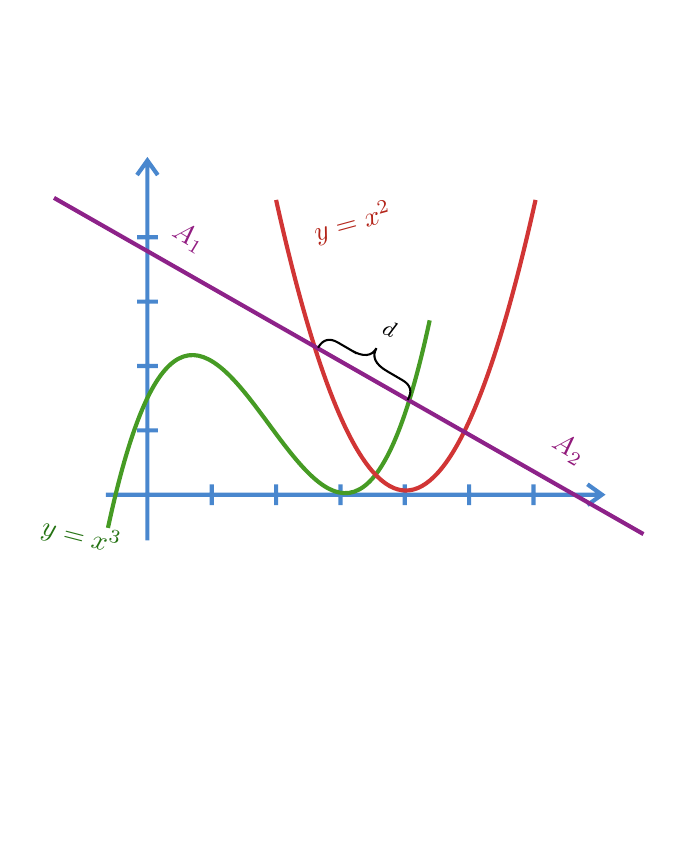
\begin{tikzpicture}[x=0.75pt,y=0.75pt,yscale=-1,xscale=1]
                    \draw [color={rgb, 255:red, 73; green, 135; blue, 206 }  ,draw opacity=1 ][line width=1.5]  (246,173) -- (485,173)(266,12) -- (266,195) (478,168) -- (485,173) -- (478,178) (261,19) -- (266,12) -- (271,19) (297,168) -- (297,178)(328,168) -- (328,178)(359,168) -- (359,178)(390,168) -- (390,178)(421,168) -- (421,178)(452,168) -- (452,178)(261,142) -- (271,142)(261,111) -- (271,111)(261,80) -- (271,80)(261,49) -- (271,49) ;
                    \draw   ;
                    \draw  [color={rgb, 255:red, 70; green, 155; blue, 36 }  ,draw opacity=1 ][line width=1.5]  (247,189) .. controls (298.67,-51) and (350.33,329) .. (402,89) ; 
                    \draw  [color={rgb, 255:red, 209; green, 53; blue, 53 }  ,draw opacity=1 ][line width=1.5]  (328,31) .. controls (369.67,217.67) and (411.33,217.67) .. (453,31) ;
                    \draw [color={rgb, 255:red, 141; green, 34; blue, 137 }  ,draw opacity=1 ][line width=1.5]    (221,30) -- (505,192) ;
                    \draw  [line width=0.75]  (391.4,127.4) .. controls (393.75,123.37) and (392.91,120.18) .. (388.88,117.83) -- (381.48,113.51) .. controls (375.72,110.15) and (374.02,106.45) .. (376.37,102.42) .. controls (374.02,106.45) and (369.96,106.79) .. (364.21,103.43)(366.8,104.94) -- (357.78,99.68) .. controls (353.75,97.33) and (350.55,98.17) .. (348.2,102.2) ;
                    \draw (286,49) node  [color={rgb, 255:red, 146; green, 29; blue, 130 }  ,opacity=1 ,rotate=-30.96]  {$A_{1}$};
                    \draw (469,151) node  [color={rgb, 255:red, 145; green, 25; blue, 123 }  ,opacity=1 ,rotate=-30.96]  {$A_{2}$};
                    \draw (234,193) node  [color={rgb, 255:red, 36; green, 114; blue, 18 }  ,opacity=1 ,rotate=-14.47]  {$y=x^{3}$};
                    \draw (365,42) node  [color={rgb, 255:red, 179; green, 35; blue, 24 }  ,opacity=1 ,rotate=-344.74]  {$y=x^{2}$};
                    \draw (382.8,93.2) node  [font=\footnotesize,rotate=-22.93]  {$d$};
                \end{tikzpicture}
                \vspace{-80pt}
                \caption{tikz draw graph example}
            \end{figure}

                \subsubsection{\texttt{tikz-cd}}
                    \begin{figure}[H]
                        \centering
                        \begin{tikzcd}
                            T
                            \arrow[drr, bend left, "x"]
                            \arrow[ddr, bend right, "y"]
                            \arrow[dr, dotted, "{(x,y)}" description] & & \\
                            & X \times_Z Y \arrow[r, "p"] \arrow[d, "q"]
                            & X \arrow[d, "f"] \\
                            & Y \arrow[r, "g"]
                            & Z
                        \end{tikzcd}
                        \caption{commutative diagram demo1}
                    \end{figure}
                    \begin{figure}[H]
                        \begin{tikzcd}[row sep=scriptsize, column sep=scriptsize]
                            & f^* E_V \arrow[dl] \arrow[rr] \arrow[dd] & & E_V \arrow[dl] \arrow[dd] \\
                            f^* E \arrow[rr, crossing over] \arrow[dd] & & E \\
                            & U \arrow[dl] \arrow[rr] & & V \arrow[dl] \\
                            M \arrow[rr] & & N \arrow[from=uu, crossing over]\\
                        \end{tikzcd}
                        \caption{commutative diagram demo2}
                    \end{figure}

                \subsubsection{\texttt{circuitikz}}
                    \begin{figure}[H]
                        \ctikzset{amplifiers/fill=cyan!15, resistors/fill=magenta!15}
                        \begin{circuitikz}[european]
                            \draw (0, 0) node[above]{$v_i$} to[short, o-] ++(1, 0) node[op amp, noinv input up, anchor=+](OA){\texttt{OA}} (OA.-) -- ++(0, -1) coordinate(FB) to[R=$R1$] ++(0, -2) node[ground]{} (FB) to[R=$R_2$, *-] (FB -| OA.out) -- (OA.out) to[short, *-o] ++(1, 0) node[above]{$v_o$}; 
                        \end{circuitikz}
                        \caption{circuit graph demo}
                    \end{figure}

        \subsection{Chemistry}
            In addition, \texttt{spAbstract} loads various chemistry-related macros, including \texttt{mhchem} and similar packages. 
            \begin{gather}
                \ce{Zn^2+
                <=>[+ 2OH-][+ 2H+]
                $\underset{\text{amphoteres Hydroxid}}{\ce{Zn(OH)2 v}}$
                <=>[+ 2OH-][+ 2H+]
                $\underset{\text{Hydroxozikat}}{\ce{[Zn(OH)4]^2-}}$
                }\nonumber
                \\\nonumber\\
                \ce{x Na(NH4)HPO4 ->[\Delta] (NaPO_3)_x + x NH_3 ^ + x H_2O}\nonumber
                \\\nonumber\\
                \ce{Hg^2+ ->[I-] HgI2 ->[I-] Hg^{II}I4^2-}
            \end{gather}
            
            \texttt{chemfig} is also provided, here are some example:
            \begin{figure}[H]
                \begin{center}
                    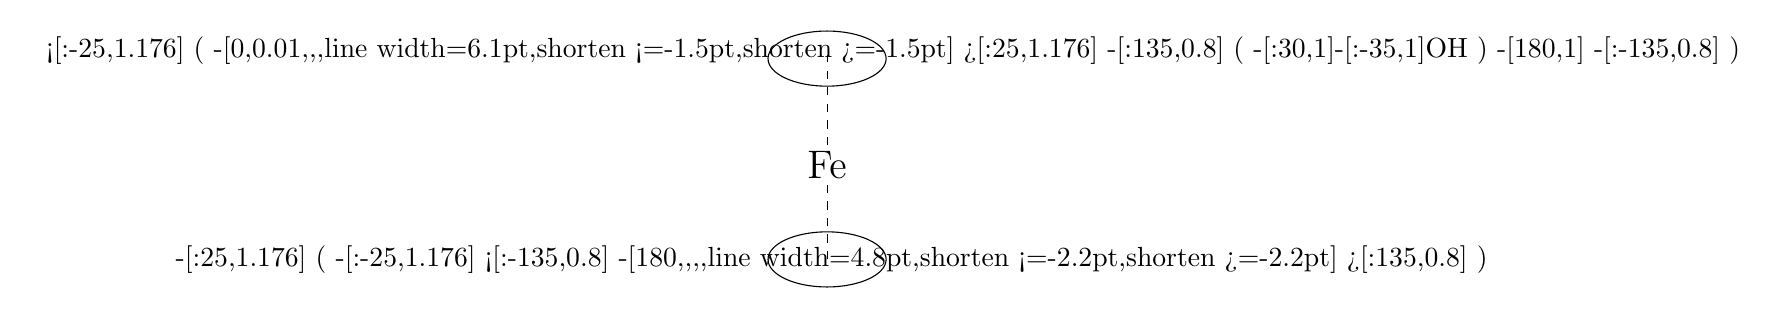
\begin{tikzpicture}
                        \node at (0.78,2.95) {\chemfig{
                                <[:-25,1.176]
                                (   
                                    -[0,0.01,,,line width=6.1pt,shorten <=-1.5pt,shorten >=-1.5pt]           
                                    >[:25,1.176] 
                                    -[:135,0.8] (
                                            -[:30,1]-[:-35,1]OH
                                            )
                                    -[180,1]
                                    -[:-135,0.8]
                                )}};
                        \node at (0,0.3){\chemfig{
                                    -[:25,1.176]
                                (            
                                    -[:-25,1.176]
                                    <[:-135,0.8]
                                    -[180,,,,line width=4.8pt,shorten <=-2.2pt,shorten >=-2.2pt]
                                    >[:135,0.8]            
                                )}};
                        \draw [dashed]  (0,1.75) -- (0,2.9);
                        \draw [dashed]  (0,0.3) -- (0,1.3);
                        \draw (0,0.3) ellipse (0.75cm and 0.35cm);
                        \draw (0,2.85) ellipse (0.75cm and 0.35cm);
                        \node at (0,1.5) {\Large Fe};
                    \end{tikzpicture}
                \end{center}
                \caption{Ferrocene, Fc. author: Lineas de ayuda, cuadricula}
                \footnotetext{\url{https://tex.stackexchange.com/questions/78275/how-to-draw-ligands-with-different-hapticities}}
            \end{figure}
            \begin{figure}[H]
                \schemestart
                \chemfig{@{a1}=_[@{db}::30]-[@{sb}::-60]@{dnl}\charge{90=\|}{X}}
                \arrow{<->}
                \chemfig{\chemabove{\vphantom{X}}{\textcolor{red}{\ominus}}-[::30]=_[::-60]
                \chemabove{X}{\textcolor{red}{\scriptstyle\oplus}}}
                \schemestop
                \chemmove{
                \draw[blue](db)..controls +(100:5mm) and +(145:5mm).. node[sloped, above]{$\textcolor{blue}{\pi}$}(a1);
                \draw[shorten <= 2pt, blue](dnl)..controls +(90:4mm) and +(45:4mm)..(sb);}
                \caption{mesomeric effect}
            \end{figure}
            \begin{figure}[H]
                \chemfig{%
                    OH-[@{l, .75}]P(=[2, .6]O)(-[6, .6]OH)-[,0.6]O-[@{r, .25}:-30]-[:25,1.176]O
                    (            
                        -[:-25,1.176](-[2, .75]N([::-18]
                            *5([,.75]-(
                                *6(-N=-N=(-[2, 0.5]NH_2)-=))--N=-)))
                        <[:-135,0.8](-[6, .75]OH)
                        -[180,,,,line width=4.8pt,shorten <=-2.2pt,shorten >=-2.2pt](-[6, .75]OH)
                        >[:135,0.8]    
                    )
                }
                \polymerdelim[height=25pt, depth=25pt, indice=\!\!3]{l}{r}
                \caption{Structure of adenosine triphosphate (ATP), protonated}
            \end{figure}

        \subsection{hlight math}
            This insight is derived from the GitHub repository \href{https://github.com/synercys/annotated_latex_equations}{\texttt{annotated\_latex\_equations}}.
            \vspace{20pt}
            \begin{equation}
                \color{purple}\underbrace{%
                \color{black}
                P\left(\tikzmarknode{mu}{\hlmath{blue}{\mu}}-\bar{X} \geqslant \tikzmarknode{t1}{\hlmath{orange}{t}} \right) \leqslant \exp \left( -\frac{2 \tikzmarknode{N}{\hlmath{xkcdHunterGreen}{N}}^2 \tikzmarknode{t2}{\hlmath{orange}{t}}^2}{\sum\limits_{i=1}^N{\left( b_i-a_i \right) ^2}} \right)
                }_{\text{Hoeffding inequation}}\nonumber
                \begin{tikzpicture}[overlay, remember picture, >=stealth, nodes={align=left, inner ysep=2pt}, <-]
                    \path (mu.north) ++ (0,+1.2em) node[anchor=south east, color=blue!67] (mu node){Expectation};
                    \draw [color=blue!57](mu.north) |- ([xshift=-0.3ex, color=blue]mu node.south west);
                \end{tikzpicture}
                \begin{tikzpicture}[overlay, remember picture, >=stealth, nodes={align=left, inner ysep=2pt}, <-]
                    \path (N.north) ++ (0,+1.2em) node[anchor=south west, color=xkcdHunterGreen!67] (N node){Samples Number};
                    \draw [color=xkcdHunterGreen!57](N.north) |- ([xshift=-0.3ex, color=xkcdHunterGreen]N node.south east);
                \end{tikzpicture}
                \begin{tikzpicture}[overlay,remember picture,>=stealth,nodes={align=left,inner ysep=1pt},<-]
                \node[anchor=south,color=orange!67, yshift=2em] (ttext) at ($(t1.north)!0.5!(t2.north)$) {Gap Length};
                \draw[<->,color=orange!57] (t1.north) |- (ttext.south) -| (t2.north);
                \end{tikzpicture}
            \end{equation}

        \subsection{lipsum and strip}
            In some case, when you encounter a long formula in twocolumn mode but you do not want devide this formula into several lines, you can use \texttt{strip} environment. Like this:

            \newpage
            \lipsum[1-3]
            \begin{strip}
                \begin{small}
                    \begin{equation}
                        \hspace{-25pt}\Gamma_{n\mathbf{Q}}^{\mathrm{ex-ph}}\left(T\right)=\frac{2\pi}{\hbar}\frac{1}{\mathcal{N}_\mathbf{q}}\sum_{m\nu\mathbf{q}}\left|\mathcal{G}_{nm\nu}(\mathbf{Q},\mathbf{q})\right|^2\left[\left(N_{\nu\mathbf{q}}+1+F_{m\mathbf{Q}+\mathbf{q}}\right)\times\delta\left(E_{n\mathbf{Q}}-E^\prime_{m\mathbf{Q}+\mathbf{q}}-\hbar\omega_{\nu\mathbf{q}}\right)\right.\left.+\left(N_{\nu\mathbf{q}}-F_{m\mathbf{Q}+\mathbf{q}}\right)\times\delta\left(E_{n\mathbf{Q}}-E^\prime_{m\mathbf{Q}+\mathbf{q}}+\hbar\omega_{\nu\mathbf{q}}\right)\right]\nonumber
                    \end{equation}
                \end{small}
            \end{strip}
            \lipsum[5-6]
            \newpage

            The \texttt{lipsum} package provides placeholder text for testing layout designs. The \texttt{strip} environment relies on the current page's typographic layout to determine the placement of its contents. If the page's layout is not suitable—such as when there are too many figures or insufficient text to divide—unexpected errors or formatting issues may occur.
\end{document}